\section{Controlling for robustness}
\label{sec:intro}
The errors in Cyber-Physical Systems (CPS) can affect both the cyber components (e.g., software bugs) and physical components (e.g., sensor failures and attacks) of a system. Under certain error models, like a bounded disturbance on a sensor reading, a system can be designed to be robust to that source of error.
In general, however, unforeseen issues will occur. 
To deal with unforeseen problems, at design time, the system must be verified to be \textit{robust} : i.e., not only does it satisfy its design specifications under the known error models, it must satisfy them robustly.
Similarly, at runtime, the system's controller must make decisions that maximize this satisfaction margin, or \textit{robustness}.
This can give a margin of maneuvarability to the system during which it addresses the unforeseen problem.
Since these problems are, by definition, unforeseen and unmodeled and only detected by their effect on the output, the notion of robustness must be computable using only the output behavior of the system.

%ATC_example
\begin{figure}[t]
\centering
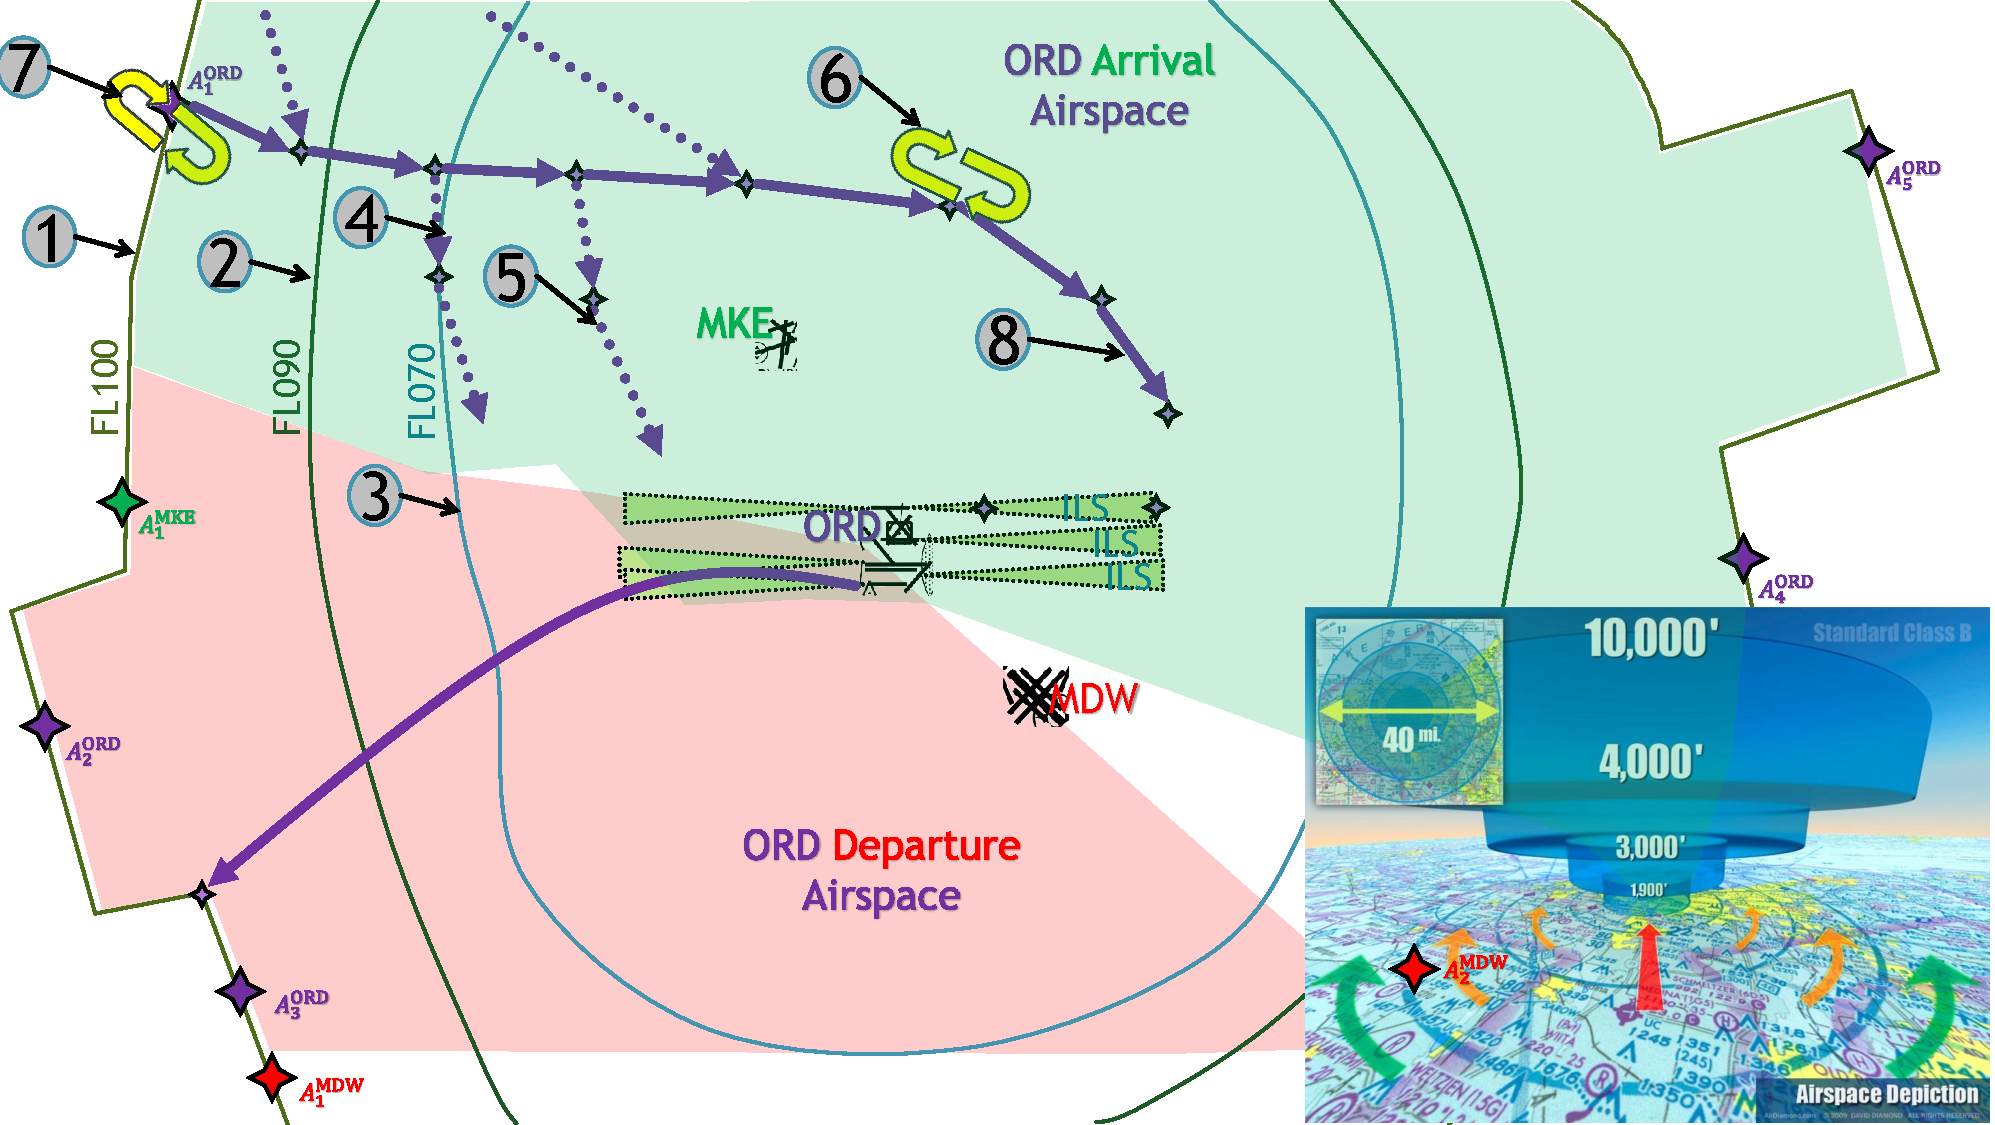
\includegraphics[width=0.49\textwidth]{figures/ATC_Example}
%\vspace{-10pt}
\caption{{\small A simplified depiction of Chicago O'Hare (ORD) airport and its airspace (40 miles radius). The numbers indicate when and where different landing rules apply. Sub-figure on the right shows the altitude rules, see text. Figure courtesy Max Z. Li, Univ. of Pennsylvania.}} 
		%\todo[inline]{Yash, double-check what i wrote in the caption. what is that sub-figure on the right?}}
\label{fig:atc_example}
%\vspace{-20pt}
\end{figure}

\begin{exmp}
%{\sf Example 1: Air Traffic Control}.
Air-Traffic Control (ATC) coordinates landing arrivals at an airport. 
ATCs have very complex rules to ensure that all airplanes, of different sizes and speeds, approach the airport and land safely, \textit{with sufficient margin to other airplanes} to accommodate emergencies and wind gusts.
Fig. \ref{fig:atc_example} depicts the airspace of Chicago O'Hare (ORD), the third busiest airport in the U.S.
The arrival airspace is divided into 3 zones with different, hierarchical, altitude floors and ceilings. 
It also shows holding zones, landing approaches, and allowable trajectories for the landing. 
The following is a subset of the rules that apply for incoming aircrafts.
\end{exmp}

\begin{enumerate}
\vspace{-5pt}
\item When an aircraft enters one of the zones (indicated by the numbers 1,2,3 in Fig.~\ref{fig:atc_example}), it must stay between that zone's altitude floor and ceiling.% E.g. zone 1 has a ceiling of 10,000 feet and a floor of 4000 feet.
\label{rule:floor ceiling}
% of has $1$, $2$ and $3$ mark three Zones, FL100, FL90 and FL70 with altitude ceilings of $10000$, $9000$ and $7000$ feet, and floors of $4000$, $3000$ and $1900$ feet respectively.
\vspace{-5pt}
\item If an aircraft approaches from the West, it must follow one of the trajectories numbered $4$ or $5$. 
%If it approaches from the East (e.g.,  in case of adverse weather), it must follow trajectory $8$.
\label{rule:waypoints}
\vspace{-5pt}
\item If the air-space is too busy, an aircraft must maintain a holding pattern in either holding zones $6$ or $7$, until some maximum amount of time expires.
\label{rule:holding}
% show two holding zones, one at the outer Zone (FL100) and the other in the inner-most zone (FL70). An air-craft could be assigned to a holding zone in case the air-space is too busy.
\vspace{-5pt}
\item A minimum separation must be maintained between aircrafts.
\vspace{-5pt}
\end{enumerate}
\begin{flushright} $\blacksquare$ \end{flushright}

How do we ensure that the ATC system satisfies these complex rules \textit{robustly}?

\subsection{The need for temporal logic}
\label{sec:morari}
The above requirements go beyond traditional control objectives like stability, tracking, quadratic cost optimization and reach-while-avoid for which we have well-developed theory.
While these requirements can be directly encoded from natural language into a Mixed Integer Program (MIP) by encoding every possibility at each (discrete) time point with integer variables, such a direct encoding can easily involve an exorbitant number of variables. For complex requirements, with many variables involved, this encoding process can also be error-prone and checking that it corresponds to the designer's intent is near impossible.
%Thus it is error-prone and checking that it corresponds to the designer's intent is near impossible.
On the other hand, such control requirements are easily and succinctly expressed in Metric Temporal Logic (MTL)~\cite{Ouaknine08_RecentResultsMTL}.
MTL is a formal language for expressing reactive requirements with constraints on their time of occurrence and sequencing, such as those of the ATC.
The advantage of first expressing the requirements in MTL is that MTL formulas are more succinct and legible, and less error-prone, than the corresponding directly-encoded MIP.
In this sense, MTL bridges the gap between the ease of use of natural language and the rigour of mathematical formulation.
%
For example, ATC rule (A) can be formalized with the following MTL formula ($\always$ means `Always', $q$ is an aircraft and $q_z$ is its altitude).

{\small
\begin{equation*}
\label{eq:rule1mtl}
\always( q \in Zone1 \implies q_z \leq \text{Ceiling1} \land q_z \geq \text{Floor1})
\end{equation*}}

Rule (B) can be formalized as follows.

{\small
\begin{flalign*}
\label{eq:rule3mtl}
\always(Busy \implies\eventually_{[t_1,t_2]} (&q \in \text{Holding-6} \, \lor \,q \in \text{Holding-7}) 
\nonumber \\
&\until_{[0,\text{MaxHolding}]} \neg Busy)
\end{flalign*}}

This says that Always ($\always$), if airport is Busy, then sometime $t_1$ to $t_2$ seconds later ($\eventually_{[t_1,t_2]} $), the plane goes into one of two Holding areas.
It stays there $\until$ntil the airport is not ($\neg$) busy, which must happen before duration MaxHolding elapses.


Once the requirements are expressed as an MTL formula, there are broadly two ways of designing a controller that satisfies the formula (fulfills the requirements).
The first method automatically creates a MIP from the semantics of the MTL formula and solves the MIP to yield a satisfying control sequence~\cite{Raman14_MPCSTL,Saha_acc16}.
See Related Work and the Experiments.
The second method, upon which this work builds, uses the \textit{robustness of MTL specifications}~\cite{Fainekos2006_TLVerifSimu,Donze2010}.
Robustness is a rigorous notion that has been used successfully for the testing and verification of automotive systems \cite{Fainekos12_Automotive,Dreossi15_RRTFalsification}, medical devices \cite{SankaranarayananF2012cmsb}, and general CPS.
Given an MTL specification $\formula$ and a system execution $\sstraj$, the robustness $\robf(\sstraj)$ of the spec relative to $\sstraj$ measures two things:
its sign tells whether $\sstraj$ satisfies the spec ($\robf(\sstraj) > 0$) or violates it ($\robf(\sstraj) <0$).
Its magnitude $|\robf(\sstraj)|$ measures how \textit{robustly} the spec is satisfied or violated.
Namely, any perturbation to $\sstraj$ of size less than $|\robf(\sstraj)|$ will not cause its truth value to change relative to $\formula$.
\textit{Thus, the control algorithm can \textit{maximize} the robustness over all possible control actions to determine the next control input.}

Unfortunately, the robustness function $\robf$ is hard to work with.
In particular, it is non-convex and non-differentiable, which makes its online optimization a challenge - indeed, most existing approaches treat it as a black box and apply heuristics to its optimization (see Related Work below).
These heuristics provide little to no guarantees, have too many user-set parameters, and don't have rigorous termination criteria.
On the other hand, \textit{gradient descent optimization} algorithms typically offer convergence guarantees to the function's (local) minima, have known convergence rates for certain function classes, usually have a fewer number of parameters to be set, and important issues like step-size selection are rigorously addressed.

\textbf{Contributions}. This paper presents smooth (infinitely differentiable) approximations to the robustness function of arbitrary MTL formulae.
The smooth approximation is proven to always be within a user-defined error of the true robustness, and this is illustrated experimentally.
This allows running powerful and rigorous off-the-shelf gradient descent optimizers.
%We demonstrate that the resulting control algorithms, which use gradient descent on the smoothed robustness, performs better than a heuristic like Simulated Annealing optimizing the original, non-differentiable robustness.
Through multiple examples, the proposed method is shown to be faster and to yield more robust trajectories than various current heuristics and MIP-based approaches. 
The results are demonstrated on a case study for an autonomous ATC for two quad-rotors, where the MIP-based approach fails to yield a satisfying controller.
While this work does not tackle the non-convexity issue directly, having an inexpensive gradient optimizer makes it possible to run an efficient multi-start optimization, increasing the chances of approaching the global optimum.

\textbf{Related work.}
Current approaches to optimizing the robustness fall into four categories: 
the use of heuristics like Simulated Annealing and RRTs~\cite{NghiemSFIGP10hscc,SankaranarayananF2012hscc,Dreossi15_RRTFalsification,Deshmukh15_IterativeApproaches}, 
non-smooth optimization \cite{AbbasF13acc}, 
Mixed Integer Linear Programming (MILP) \cite{Raman14_MPCSTL,Saha_acc16}, 
and iterative approximations \cite{AbbasATVA11_LinFalsification,Abbas14_MTLDescent}.
Black-box heuristics are the most commonly used approach: for example, Simulated Annealing~\cite{NghiemSFIGP10hscc}, cross-entropy \cite{SankaranarayananF2012hscc} and RRTs~\cite{Dreossi15_RRTFalsification}.
The clear advantage of these methods is that they do not require any special form of the objective function: they simply need to evaluate it at various points of the search space, and use its value as feedback to decide on the next point to try.
A significant shortcoming is their lack of guarantees as explained earlier.
% they offer little to no guarantees of convergence to local minima, and their convergence rates are often not known. 
%They also use many `magical' parameters that are heuristically set and may affect the results significantly.
%%The same is true of deterministic heuristics \cite{zutshi_trajectory_2013}, albeit they tend to be more transparent to the user and can be better tuned.
Because the robustness is non-smooth, the work in \cite{AbbasF13acc} developed an algorithm that decreases the objective function along its sub-gradient. 
This involved a series of conservative approximations and was restricted to the case of safety formulae.
In \cite{Raman14_MPCSTL}, the authors encoded the MTL formula as a set of linear and boolean constraints (when the dynamical system is linear), and used Gurobi to solve them.
%The resulting MILP and used a Mixed Integer Linear Program (MILP) has $O(N\cdot|P|)$ binary variables (where $N$ is the number of samples in the trajectory over which we optimize and $|P|$ is the number of predicates, and $O(N\cdot |\formula|)$ continuous variables.
MILPs are NP-complete, non-convex, and do not scale well with the number of variables. 
The sophisticated heuristics used to mitigate this make it hard to characterize their runtimes, which is important in control - see examples in \cite{Raman14_MPCSTL} and this paper. 
In general, MILP solvers can only guarantee achieving local optima.
Note also that \cite{Raman14_MPCSTL} requires all constraints to be linear, so all atomic propositions must involve half-spaces ($p: a'x\leq b$), which is not a restriction in the current work.
The work closest to this paper is \cite{AbbasATVA11_LinFalsification,Abbas14_MTLDescent}.
There, the authors considered safety formulas, for which the robustness reduces to the minimum distance between $\sstraj$ and the unsafe set $U$.
By sub-optimally focusing on one point on the trajectory $\sstraj$, they replaced the objective by a differentiable indicator function for $U$ and solved the resulting problem with gradient descent.
\todo[inline]{say something about saha,julius}
The use of fast smooth approximations of robustness circumvents most of the above issues and gets closer to real-time control by robustness maximization.




